In this chapter, the background of data clumps will be discussed. A formal definition of code smells and  of data clumps will be presented ( sections \ref{sec:code_smell} and \ref{sec:data_clump_def}). ChatGPT will be discussed in section \ref{sec:chatgpt}. Also, the data clump type context format will be discussed in section \ref{sec:data_clump_format}. The Language Server Protocol which used by to refactor data clumps more easily is explained in section \ref{sec:lsp}. In the end, related research will be discussed (see section \ref{sec:related_research}). 
\section{Code smells}\label{sec:code_smell}

The term \enquote{Code smell} is a term suggested by Kent Beck in \cite{fowler2019refactoring} for source code that may need refactoring. If the refactoring is not performed timely, the costs of maintenance of the source code and the software project can be higher and the efficiency of implementing changes is reduced. Some examples of code smells include unclear variables names, large classes, large method, missing documentation or code duplicates. Another possible code smell are data clumps. 

\section{Data clumps}\label{sec:data_clump_def}
The term \enquote{Data Clump} was coined by Martin Fowler as one possible code smell that can occur in source code. He describes data clumps as follows:

\begin{displayquote}
Data items tend to be like children: They enjoy hanging around together around in groups. Often you will see
the same three or four data items together in lots of
places: fields in a couple of classes, parameters in many
method signatures. \cite{fowler2019refactoring} 
\end{displayquote}

This definition is somewhat imprecise. It is not specified whether three or four data items are necessary. Also, \enquote{a couple of classes} and \enquote{in many method signatures} do not define concrete numbers. The author suggests checking whether the removal of one data clump item would have a significant effect on the coherence of the code.

A more precise and algorithmic definition of \enquote{data clumps} is provided by \cite{zhangImprovingPrecisionFowler2008}. They say a data clump  can be defined on the field or method-parameter levels. 
To be a method parameter data clump, a group of at least three variables must appear in multiple methods. Those variables must be duplicated, meaning they share the same name and data type. However, the inner order of the group does not need to be the same. 

These conditions often need to be more relaxed. For instance, methods can be inherited and overridden so that a group of parameters may appear in each derived class, thereby fulfilling the definition of a method parameter data clump. Since (except for the identifiers of the parameters) an overriding method must be the same as the overridden method, they are not considered data clumps.

For field data clumps, similar conditions apply. There must be at least three fields that appear in more than one class, and the names and data types of the variables must be the same, while the inner order may be different. Since in most programming languages, a field can have an additional access modifier (e.g., \textit{private}, \textit{static} etc. ), the access modifier should also be included to determine whether two groups of variables are identical and hence a data clump.  

The definition might also need to be more relaxed for both method and field data clumps. Two variables that have the same name but a compatible type in at least one direction  (e.g., \textit{int} and  \textit{double}), would be disregarded as a data clump according to the formalized definition. However, some would regard them as a data clump.

Also, modification of a variable's identifier might not change its meaning. For instance, typos can happen, or synonyms can be used so that an automatic algorithm might not discover the connection between two variables but requires knowledge of the semantics of the source code. \cite{zhangImprovingPrecisionFowler2008}


To conclude, the core definition of a data clump is clear. However, this definition still leaves out some edge cases that require a semantic understanding of the source code. 

An example of a data clump is shown in listing \ref{lst:math_stuff_java}
\begin{figure} [htbp!]
			\lstinputlisting
			[caption={Some operations on vectors},
			label={lst:math_stuff_java},
			captionpos=b,language=java, basicstyle=\footnotesize, tabsize=2, showstringspaces=false,  numbers=left]
			{figures/chapter2/dataClump/MathStuff.java}
		\end{figure}



Listing \ref{lst:math_stuff_java} contains three methods that execute some vector operations (calculation of length, sum of coordinates, and the maximum coordinate). 


It can be seen that  the snippet contains a method parameter data clump since the variables \textit{x}, \textit{y}, and  \textit{z} occur thrice.  These variables might be called \textbf{data clump items}
  
\subsection{Refactoring data clumps}
Fowler suggests two  steps to refactor a data clump:

In the  \textbf{Extract-Class}-step, a class with fields for each data clump item is extracted. A class for this purpose might already exist so that it can be re-used.

In the second step, \textbf{Preserve Whole Object} or \textbf{Introduce Parameter Object} might be applied. This means that the signature of the method is changed so that the extracted class replaces the data clump items, and all references to the method are changed accordingly.


To illustrate the suggested data clump refactoring process, listing \ref{lst:math_user_java} shows how the methods in \ref{lst:math_stuff_java} can be used. 


  \begin{figure} [htbp!]
			\lstinputlisting
			[caption={Some operations on vectors},
			label={lst:math_user_java},
			captionpos=b,language=java, basicstyle=\footnotesize, tabsize=2, showstringspaces=false,  numbers=left]
			{figures/chapter2/dataClump/MathUser.java}
	\end{figure}

In the first step, a new class can be extracted, which contains all data clump items as fields. It should also contain setters and getters to access the fields in an encapsulated manner. The class should be named so that its purpose is clear. Listing \ref{lst:coordinate_java} shows how such a class may look like. 

  \begin{figure} [htbp!]
			\lstinputlisting
			[caption={ Resulting Coordinate class},
			label={lst:coordinate_java},
			captionpos=b,language=java, basicstyle=\footnotesize, tabsize=2, showstringspaces=false,  numbers=left]
			{figures/chapter2/dataClump/Coordinate.java}
		\end{figure}

In the second step, a parameter object is introduced that replaces the three previous data clump items in each of the three methods of the \textit{MathStuff} class so that the signature only contains one parameter of type \textit{Coordinate}. Also, the calls in \textit{MathUsage} are refactored to reflect that change ( listing \ref{lst:math_stuff_refactored_java} and \ref{lst:math_user_refactored_java}). 

  \begin{figure} [htbp!]
			\lstinputlisting
			[caption={ Resulting Coordinate class},
			label={lst:math_stuff_refactored_java},
			captionpos=b,language=java, basicstyle=\footnotesize, tabsize=2, showstringspaces=false,  numbers=left]
			{figures/chapter2/dataClump/MathStuffRefactored.java}
		\end{figure}
  \begin{figure} [htbp!]
			\lstinputlisting
			[caption={ Resulting Coordinate class},
			label={lst:math_user_refactored_java},
			captionpos=b,language=java, basicstyle=\footnotesize, tabsize=2, showstringspaces=false,  numbers=left]
			{figures/chapter2/dataClump/MathStuffRefactored.java}
		\end{figure}

\subsection{ Data clumps Type Context }\label{sec:data_clump_format}

The \textbf{Data clumps Type Context} \cite{dataclump_type_context} is developed by Baumgartner et al. to establish a standard for reporting data clumps.

An example of the Data clump type context can be seen in listing \ref{lst:data_clump_type_context_example}. Only a subset of the formate will be discussed here because of space reasons.

  \begin{figure} [htbp!]
			\lstinputlisting
			[caption={ Resulting Coordinate class},
			label={lst:data_clump_type_context_example},
			captionpos=b,language=java, basicstyle=\footnotesize, tabsize=2, showstringspaces=false,  numbers=left]
			{figures/chapter2/data_clump_type_context_example.json}
		\end{figure}

The format consists of three layers. In the outer layer which is left out here, general project information is defined: For instance, the programming language or the location of the project. Also the number of methods, classes, and the number of detected data clumps can be obtained in this general part. 

In the next layer, each detected data clump is mapped with a unique key (l. 4).

The detected data clumps are described as a link between two files. These files might be identical if the data clumps are located in the same file. Here one has to differ between the \enquote{from-part} and the \enquote{to-part} which represent the two nodes in the data clump graph. For instance \enquote{from\_file\_path} indicates the location of the one part of the data clump, while \enquote{to\_file\_path} provides the path to the opposite end. 

A similar principle is apllied to the classes in which a data clump is located. Because a class name might not be unique, not only the names of the two classes but also unique ientifier of those classes are provided (l. 9-10 and 14-15).

The information about the methods of the data clump )l. 11, 12, 16, 17) is optional. if one part of the data clump is a field-to-field data clump, no method is involved so the respective part would be \textit{null}.

The field \enquote{probability} can be used by probabilistic data clump detection tools to indicate the probability that the detected data clump is indeed a data clump. For purposes of this master thesis, it will be ignored. 

In lines 19-42, each variable that is part of the data clump is  described. Here only one variable is listed although for a data clump there must be at least three variables. As for the data clump itself, the individual variables are separated into  a \enquote{from-part} and a \enquote{to-part}. The former is implicitly defined (l.~20-25, 38-42), while the latter has a specifically named sub object \enquote{to\_variable} (l. 27-37). For each variable, the name (l. 22 and l. 28)) and the data type (l.~23 and l. 29) is provided. As for the general data clump, a probability is given whether the variable is indeed part of a data clump (l. 24). As mentioned above, this information will be ignored.  Additionally modifiers like \enquote{private}, \enquote{final} etc. are also stored. 

In order to find the variable in the source code, detailed location information is needed. In source code, the line number (l.~32 and l.~39) and the column number (l.~33 and l.~40) is required . To avoid any ambiguity, the end position of the variable is saved too. Both numbers are one-index-based meaning that the first line is 1 and the first column is also 1. 


\section{ChatGPT}\label{sec:chatgpt}

ChatGPT \cite{ChatGPT_url} is a \ac{LLM} developed by OpenAI and released in November 2022. As a \ac{LLM}, ChatGPT can interpret user queries and return an appropriate response. 

A query can be a question or a prompt directing ChatGPT to answer a question or provide some output. The range of topics ChatGPT can help with is basically unlimited. For instance, ChatGPT can help with math, history, politics, or coding topics. ChatGPT can also understand programming language and therefore, help developers to code. Since September 2023, ChatGPT can also process images \cite{ChatGPT_image}. However, it must be noted that ChatGPT may not always provide accurate responses since it is, in the end, just a language model without knowledge about the inherent meanings of its responses. 

The usage of ChatGPT is nevertheless somewhat restricted. For instance, content regarded as hate speech or used for illegal purposes will be suppressed.

Another essential feature of ChatGPT is the ability to store conversations. A conversation is a collection of queries and linked responses sent to ChatGPT. Using conversations, a user can refer to a previous query or response in a later query. For instance, if ChatGPT makes a mistake or misinterprets a query, a user can send another request connected to the previous request and point out the mistake or give more context, helping ChatGPT auto-correct itself. 

ChatGPT can be used via a browser or via an API. Using ChatGPT via the browser is free although restricted. A paid version is available that is faster and uses an improved model that supports the beforementioned image generation and other features not relevant for this master thesis.  Using the API requires a payment based on used token. A token is approximately a word but a detailed definition of a token is difficult to specify. 

Figure \ref{fig:chatgpt_browser} illustrate how ChatGPT can be used in the browser.
\begin{figure}
    \centering
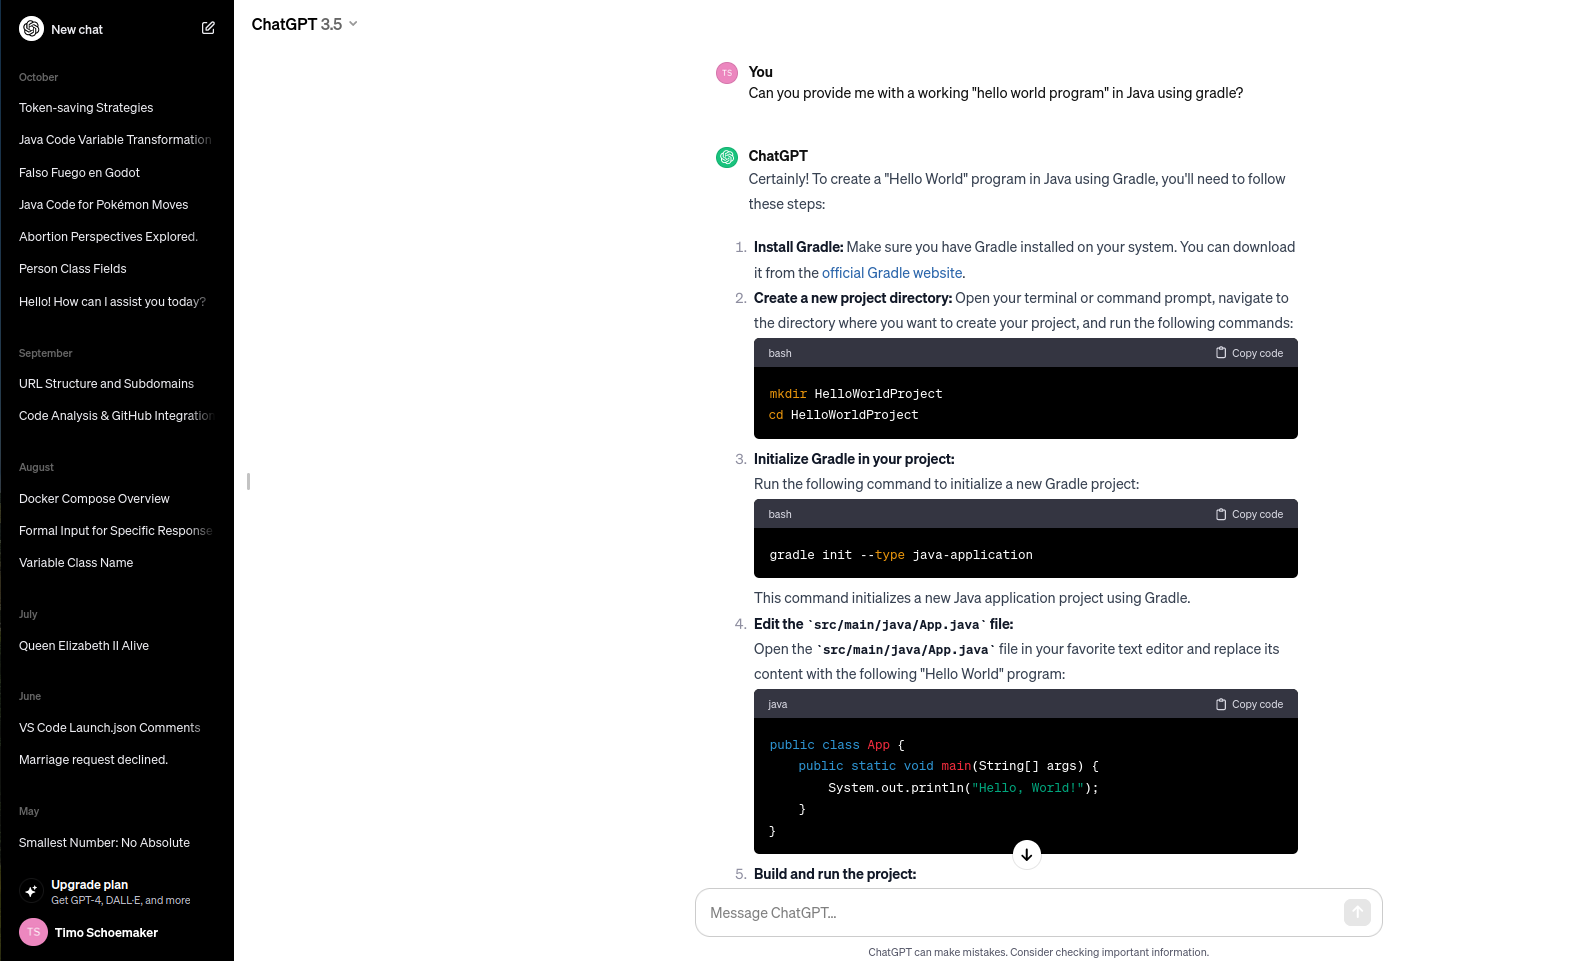
\includegraphics[width=\columnwidth]{figures/chapter2/chatgpt_browser.png}
    \caption{ChatGPT in the browser}
    \label{fig:chatgpt_browser}
\end{figure}
In the main panel that encompasses the most area of the figure, a chat is visualized. This is the the chat with the ChatGPT model. The queries are headlined with \textit{You} and the responses with \textit{ChatGPT}. In this example, ChatGPT is asked to create a hello world program with gradle. As a response, the model returned code blocks which the user can simply copy and use. Also descriptions are provided to explain the context and usage of the code.

    On the right side, all conversation with ChatGPT are listed. For instance, there is a conversation about \enquote{IntelliJ PSI Modification Fix}. A user can have multiple independent conversations where each has it own context. 

\subsection{ChatGPT API}
In order to use ChatGPT \ac{API}, a user has to create an OpenAI account and deposit financial information so that the user can be charged. Each request to the API consumes a certain amount of tokens dependent on the query. 

A token is the smallest unit used by ChatGPT to process a query. For instance, a token could be one english word, o syntactical part of a programming language, a number or a similar independent part of a query. According to OpenAI, a token is 3/4 of a word so that 100 tokens are about 75 words. However, this is just an estimate for natural language texts in the English language. 

The \ac{API} itself used JSON combined with HTTPS. For the purpose of this master thesis, only a subset of the available means to use the \ac{API} will be explained because the whole \ac{API} would be too complex and irrelevant. 

\subsubsection{Query}
Listing \ref{lst:chatgpt_api} shows how an \ac{API} query may look like if it used via \textit{curl} which is a tool perform HTTP requests:
 \begin{figure} [htbp!]
			\lstinputlisting
			[caption={ Example query to ChatGPT  \cite{ChatGPT_url}},
			label={lst:chatgpt_api},
			captionpos=b,language=java, basicstyle=\footnotesize, tabsize=2, showstringspaces=false,  numbers=left]
			{figures/chapter2/chatgpt_api.json}
		\end{figure}
 

Since ChatGPT uses \ac{JSON} for communication, the content header of HTTP  must be set to \enquote{application/json} (l. 2). Afterwards, a token must be provided to ChatGPT (l. 23). This  token must be generated on the OpenAI website and will be used to connect the query to an OpenAI account so that the user can be charged properly- The token should remain secret and may not be disclosed (e.~g. via \ac{VCS}) 

Then, the actual query is defined (l. 4-24.)Firstly, the model is defined (l. 5). OpenAI provides multiple models that have different advantages and disadvantages. For instance, a newer model like \textit{gpt-4} has more capabilities but is more expensive. 

Afterwards, the actual messages are provided (l. 6-24). Each message is a tuple of a \textbf{role} and a \textbf{content}. The content of a message is the input or output provided to or by ChatGPT. 

The role of a message indicates the source of a message. If the content of the messages comes from a user, the role should be \enquote{user} (l. 12). A reply for a query is defined as the role \enquote{assistant} (l. 16). The system role is a more specific role and can be used to include further context for ChatGPT without eliciting a response (l. 8)

ChatGPT is stateless. This means that the token id explained above is solely used for accounting purposes and not to store the queries reliably. As a result, if one wants to hold a conversations similar to the browser version,  not only all previous messages from the user must be sent to ChatGPT, but also all replies and the messages of the system role. This should be considered while using the OpenAI \ac{API} because the number of required tokens can strongly increase for longer conversations.

\begin{figure}
    \centering
    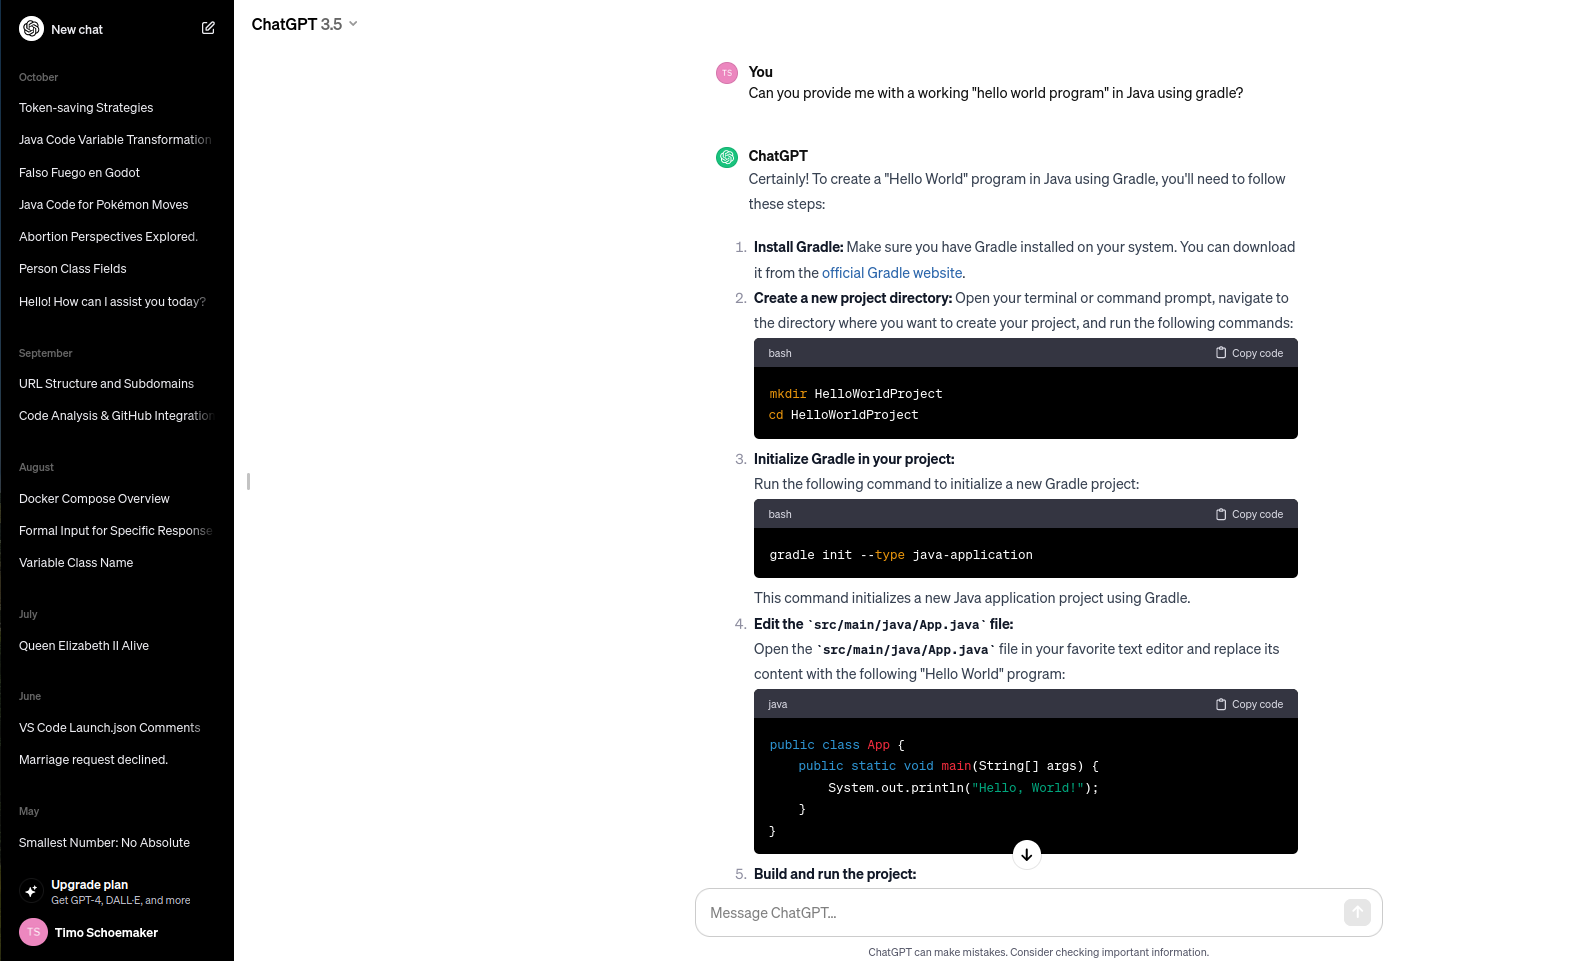
\includegraphics[width=\columnwidth]{figures/chapter2/chatgpt_stateless.png}
    \caption{Visualization of statelessness of ChatGPT. Rectangles are queries by the user. Ellipses are replies by ChatGPT}
    \label{fig:chatgpt_stateless}
\end{figure}


Figure \ref{fig:chatgpt_stateless} visualize this issue. Here, the user ask the ChatGPT API to find all data clump in a java file \textit{(request 1)}. ChatGPT respond with some data clumps. These might not be all data clumps so that a follow-up request might improve the results \cite{10062688}. Therefore, the user sends another request \textit{(request 2)} to instruct the model to find more data clumps. However ChatGPT responds with a general stating that it does not know the content of the file \enquote{MathStuff.java}. This is the result of the statelessness which requires that the user always send the whole context with each query. In \textit{request 3}, the context is provided so that ChatGPT acurately responds by finding another data clump.

Since follow-up request make only sense if ChatGPT has already responded, the whole original request, the reply by ChatGPT, and any previous conversation must be provided which can have a large impact on costs and rate limits. 

\subsubsection{Response}

The response of the ChatGPT \ac{API} based on listing \ref{lst:chatgpt_api} is displayed in listing \ref{lst:chatgpt_api_response}.
 \begin{figure} [htbp!]
			\lstinputlisting
			[caption={ Example query to ChatGPT  \cite{ChatGPT_url}},
			label={lst:chatgpt_api_response},
			captionpos=b,language=java, basicstyle=\footnotesize, tabsize=2, showstringspaces=false,  numbers=left]
			{figures/chapter2/chatgpt_api_response.json}
		\end{figure}

In the lower part of the listing (l. 13-19), meta information is provided. This includes the response generation time (l. 12), the used model for the response (l. 14), an id for the response (l. 13).

In order for clients to calculate the costs of using ChatGPT, each response also includes how many tokens have been used by the prompt (l. 18), by the response (l. 17), and the total number of tokens (l. 19).

In the upper part of the response (l. 1-11), the actual response is provided. The response is an array of so-called choices (l. 2~-~11). Each choice consists of the actual message (l.~ 6-8), which itself consists of the message content (l. 7) and the role of  the content (in most cases this would be \enquote{assistant}).

The \enquote{finish\_reason} indicates how the \ac{LLM} has finished on the prompt. If the value is \enquote{stop}, the prompt was executed without faults so that the response is valid. If the value is \enquote{length}, the output would esceed the maximum token limit, so that the output will be incomplete. The value \enquote{content\_filter} indicated the OpenAI censured the requests because it violates the terms of use of OpenAI. \cite{ChatGPT_url}
\subsection{Advantages and Challenges on using Large Language Models}\label{sec:llm_challenges}

While using  \ac{LLM} for refactoring bring many advantages  and possibilities, using \ac{LLM}  successfully can be challenging. The advantages and disadvantages will be discussed in this subsection. A \textbf{traditional algorithm} as used in this section means any manual refactoring algorithm (e.~g.,~ refactoring data clumps by extracting a class, removing and introducing parameters in methods, and updating all references)

\subsubsection{Advantages}

First of all, large language models are very flexible. A normal refactoring algorithm needs to consider many situations. For instance, an algorithm that modifies the method signature in a class might not work on an interface. A large language model does not need to be adapted to all edge cases but often finds a suitable solution to a problem because it is not restricted to a specific refactoring process, 

Additionally, a \ac{LLM} is more similar to a human as it more  \enquote{creative}. While it is still a computer model and does not win the Turing-Test \cite{turing_test}, a \ac{LLM} can refactor code in a manner more closely as a human being would do. For instance, it can suggest class names that are related to the topic of the class, which a human being would also consider, while traditional algorithm would use placeholder names, concatenation of fields names or other simple name construction algorithms. 

Large language models are also extensible. For instance, if another programming language is used, an \ac{LLM} can be easily adapted while a traditional refactoring approach would require more effort to be language-agnostic.

Moreover, a \ac{LLM} can refactor the code in more ways than instructed. While  a model can be  specifically instructed to refactor data clumps, it might also correct formatting errors, spelling mistakes, or other code smells. While the focus of this master thesis will be on data clumps, other code smells are important too and might be more serious. Using a  \ac{LLM} allows developers to fix more code smells, without developing and testing more tools to refactor multiple code smells. As they are better to understand the context of the code than a traditional algorithm, the quality of the code can therefore be improved. 

Furthermore, \ac{LLM} can adapt to the coding style of the source code. If for instance, the source code used the \enquote{snake\_case} or the \enquote{pascalCase} naming convention, the model can detect this convention and use it for its own refactoring (e.g. creating new methods, variables or classes). A traditional approach would need to be configured for each project to use the right convention so that the generated code might look more artificial as it does not fit to the rest of the code.


\subsubsection{Disadvantages}

First of all \ac{LLM} are not trustworthy. They are often confident in their answers which nevertheless are wrong. This confidence can often be broken by asking subsequent questions which lead the \ac{LLM} to rethink the answer. however, doing this in an automatic way is challenging.

Additionally, \ac{LLM} use randomness in their answers which means that the same query can result in different replies. The factors influencing the reply are generally not known and should not be assumed. As a result, requirements regarding a specific output format, may be ignored by the model so that developers using a \ac{LLM} must always consider how to parse non-adhering output. 

Furthermore, \ac{LLM}s are usually black boxes. They do not give hindsight on how they came to a specific reply. While they can explain their reasoning, it is not possible to check the exact thought process.
While a query can consists of multiple parts, conditions, or requirements, a \ac{LLM} will not always adhere to all of these. It may weight some requirements, ignore other or interpret them wrongly so that the result is unexpected. A \ac{LLM} may also come to an intermediate result that it will not show at the end even though the intermediate result was correct or requested. Also no sources of the information is provided. 

Moreover, \ac{LLM}s do not have access to the latest information about a topic. They cannot access external sources like current news  and up-to-date documentation. Instead they employ a so-called cut-ff date. Only information before that cut-off date will be used. As of the time of writing this section, the cut-off date for ChatGPt is April  2023. However, the release was several months later.  

There also security issues with using  \ac{LLM} like ChatGPT. If a model is asked to generate or refactor code, one cannot trust that the code is safe to use. As a result of the cut-off date, the code might use operations that are considered deprecated or even unsafe to use because security vulnerabilities have been detected in the meantime. As a result, the developer needs to verify whether the code is safe to use which is another burden. 

Furthermore, it is not out of the question that a malicious attacker might change the query or the reply of a \ac{LLM}. Therefore, using such a model might be a feasible way to hack systems or create damage which is difficult to detect and prevent.

Lastly, also costs and capacity considerations needs to be observed. For large projects, a \ac{LLM} might be too costly because  the costs are often based on the input size. Therefore, the use of large language models should be adequately prepared so that as much costs as possible can be saved.  
\subsection{Consideration while using large language models}
In order to use a \ac{LLM} more effectively, the prompts and queries need to be modeled in a specific manner so that they are interpreted correctly. While deviating from these manners may still produce correct results, it nevertheless increases the risk of wrong results. The following tips were derived from the OpenAI documentation \cite{ChatGPT_url} and hence apply only to ChatGPT. Generally speaking. However, many recommendations will work for other \ac{LLM} too because they will help to make the prompt more clearly and prevent misunderstanding:

\subsubsection{Separate instruction and input}
Many queries to \ac{LLM} include an instruction and an input. For instance, a query to find and refactor data clumps could  provide the source code containing the possible data clumps \textbf{(input)}. The instruction could be the query \enquote{Find and refactor all data clumps in this source code}. 

OpenAI recommends that the instructions and input be separated as distinctive as possible. It suggests enclosing the input in a block of \textit{"""} or \textit{\#\#\#} to mark what the input and what the instruction is clearly.

\subsubsection{Provide detailed context and how the model should respond}

When generating a reply to a query, a language model will use the available context to process the query and generate an output that attempts satisfy the user's need. This means that every bit of relevant information can help the language model to generate a better response.

On the contrary, providing irrelevant information can increase the chance of wrong responses, so the creator of a query must always consider what to include in a query and what not. 

In the context of data clump refactoring, the query should include the content of the source code and the programming language. However, files that cannot have data clumps (e.g., configuration files) should not be included.

An instruction for refactoring data clumps should state that only the refactored source code files should be returned without providing explanatory texts or other information, as they can hinder the parsing of the output. 

When using the \enquote{gpt-4-1106-preview} or \enquote{gpt-3.5-turbo-1106} model of the OpenAI-\ac{API}, developers can force the model to response in \ac{JSON}. hence, the output can be made more predictable and easier to control. A request using this mode must include the term \enquote{\ac{JSON}}. It should however be noted, that the precise structure of the \ac{JSON} returned may still differ from the request. 

\subsubsection{Politeness is not necessary}

Polite words like \enquote{please} or \enquote{thank you} are expected in human conversations. However, a  \ac{LLM} will ignore these words that are often referred to as \enquote{filler} words, or their effect will be marginal. Since costs are an important part of the usage of \ac{LLM}, these words are often unnecessary. \cite{bsharat2023principled}.

\subsubsection{Avoid using prohibition but suggest alternatives}

Providing prohibitions to a \ac{LLM} may sound like a valid approach to restrict certain outputs. However, they can degrade the quality of the results. For example, if a \ac{LLM} has found a solution that violates a prohibition, it does not know how to proceed. 

In contrast, giving positive instructions, the \ac{LLM} can better determine how the user expects the output so that the quality is increased.

For instance, instructing a \ac{LLM} to not write informally can result to worse outputs than an instruction to use formal language because formal language is better defined than the negation of informal language. \cite{prompt_engineering_jonathan}

\subsubsection{Provide rewards or punishments to the LLM}

While a \ac{LLM} is not a human, its result can be influenced by rewards or punishments. For instance, the authors in \cite{bsharat2023principled} claim that promising the model a monetary amount, can lead to better results. 

Similarly, informing the model that certain results will be punished, can decrease the likelihood that these results will be returned. \cite{bsharat2023principled}
\begin{comment}
\subsection{Cost reduction}

Many \ac{LLM} are not for free but must be paid based on usage or other factors. Even if a \ac{LLM} is free, there are many restrictions for the data to be processed by the model, so special care needs to be taken to reduce the data size as well as possible.  The cost might already be reduced by following the steps in section \ref{sec:prompt_engineering}. Nevertheless, there are other factors that will be outlined:
\end{comment}

\subsubsection{Chain-of-Thought Prompting}\label{sec:chain of thought}

Another approach to improve the results from \ac{LLM} like ChatGPT is to separate a query into interconnected sub queries that lead to a chain of thought. This can be compared to human thinking process because a human alone tries not to solve a problem at once but breaks it downs into simpler problem that are still connected to but easier to solve. \cite{Wei2022ChainOT}

For instance, a query to find and refactor data clumps can be separate into a detection query and a refactoring query. These sub-queries can be further divided into a query for each file or for all files in a single directory. As a result, not one a single query needs but multiple queries. 

This is useful if a human is reviewing the output from a \ac{LLM} since obvious errors can be spotted more easily if the task is divided into multiple  step. However, it is more challenging for an automated tool since it cannot find errors in the same way. 

Furthermore, one should consider that each queries requires further overhead so that the performance might be impacted more negatively. 
\section{Language Server Protocol} \label{sec:lsp}
The \ac{LSP}  \cite{lsp_website} is a protocol developed by Microsoft to create a language-independent interface for code-related operations. 
The \ac{LSP}  describes a server and a client who communicate to each other using the JSON-Remote-Process-Call protocol \cite{json_rpc}. 

In general, the client can be anything that works with source code but has no detailed knowledge of a specific programming language. For instance, an \ac{IDE}, an editor or a refactoring tool can be described as a client.

The client starts a server based on a programming language. The server has a inherent knowledge of one ore more programming languages and can provide source-code-related functionality. For instance, the server can rename a variable, find the usages of a method, or inform the client about compiler errors. 

Initially, client and server share some information to set-up. This includes the path to the project that the server should load and information about what functionality each of them support. These functionalities are named \textit{Capabilities}. For example, the server can announce that it supports renaming variables while the client show error messages. Hence, server and client can interact in a manner such that no unsupported messages are transferred.

Figure \ref{fig:lsp_usage} illustrates how the \ac{LSP} works in practice after the initialization process. 
\begin{figure}
    \centering
    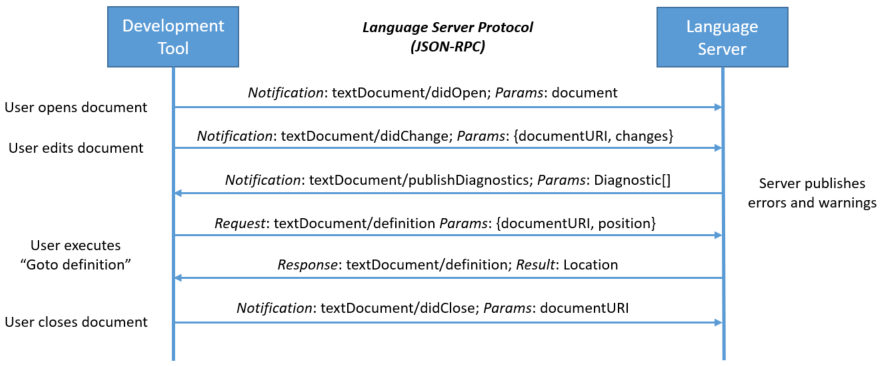
\includegraphics{figures/chapter2/language-server-sequence.png}
    \caption{Example usage of the Language Server Protocol}
    \label{fig:lsp_usage}
    \cite{lsp_website}
\end{figure}

After the server has successfully started by the client, a user can open a document (e.g. source code file). The request to open the document is submitted to the server. From now one, the server may not rely on the file system since that might be not the current version of the opened document. 

The client can now inform the server about some changes (e.g. adding a new method). The server can in the meantime inform the client about syntactical errors which the client might show to the user of the client.

Afterwards, the client requests the definition of a method or variable, and the server returns a response with the requested data.

In the end, the client can save the document and notify the server that the document was closed which means that the physical file of the document represents the current version of the document again. 



\section{Related Research}\label{sec:related_research}
The problem of data clump detection and refactoring is addressed in multiple papers. Also the  use of large language models in software development is a fairly recent rearch topic. In this section, research to both topics will be outlined: 

\subsection{Related to data clumps}
Baumgartner et al.  developed a live code smell detection plugin for IntelliJ that can detect, report, and refactor data clumps without significantly impacting performance. However, the tool is semi-automatic, meaning the developer must still actively approve the data clump refactoring and suggest a suitable class name for the extracted class. \cite{BaumgartnerAP23}

As outlined in section \ref{sec:data_clump_def}, the definition of data clump by Fowler \cite{fowler2019refactoring} is somewhat ambiguous because no clear criteria to determine data clumps is established. Zang et al. \cite{zhangImprovingPrecisionFowler2008} creates a more algorithmic approach to determine whether a data clump exists. This approach is also explained in section \ref{sec:data_clump_def}. The authors also provide more precise definitions of other code smells like \enquote{message chains} or \enquote{speculative generality}. By interviewing four software development experts about the code smell definitions the authors developed, they find that their new data clump definition receives relatively more disagreement than other definitions, which the authors explain are the results of not covering edge cases in the definitions. 


Hall et al. analyzed the impact of code smells (including data clump) on the occurrence of faults in three open-source software projects. They find that data clumps have a mixed correlation to faults because, in two of the three projects analyzed, the correlation of data clumps per \ac{LOC} to detected faults is negative for two projects and positive for one project. This rejects their hypothesis that data clumps do not affect faults, and the authors suggest that the application domain and the development context need to be considered before the time-consuming refactoring of data clumps since their impact is not predictable.  \cite{hallCodeSmellsHave2014}

\subsection{Related to large language models in software development}

White et al. \cite{White2023ChatGPTPP} outline how ChatGPT can be used in software development to improve the worklflow of developers. This includes  exploration of requirements, removing ambiguity in technical specification, or describing source code. The authors suggest specific prompts to elicit a suitable response from ChatGPt.

In case of refactoring, the author suggest that ChatGPT is able to refactor code with multiple prompts. For instance, ChatGPT can refactor based on a well known design pattern name, multiple examples on how to refactor the code, or a more lengthy requirements description. The exact success of each prompt is however dependent on how ChatGPT is trained and should be scrutinized manually. 

Cao et al. \cite{cao2023study} focus on using ChatGPT for fixing deep learning programs. Those are programs that cannot be understood only by their source code alone, but are are largely influenced by underlying data like  neural networks etc. This makes finding faults more difficult. The study finds out that ChatGPT can find code smells and detect faults. Without giving instructions however, ChatGPT will tend to return code smells and outdated API calls while not finding other bugs. 



